%! Author = gramic
%! Date = 01.05.24

% Preamble
\clearpage
\KOMAoptions{paper=A3,paper=landscape,pagesize, DIV=20}
\recalctypearea
\begin{flushleft}
    \subsection{Protokollierung}
    \begin{table}[H]

\resizebox{\columnwidth}{!}{%

\begin{tabular}{lrllll}
\toprule
Art & Test Case Nr. & Test Case & Erwartetes Ergebnis & Eingetretenes Ergebnis & Begründung \\
\midrule
Basistests & 1 & Connection & \begin{tabular}[c]{@{}l@{}}Verbindung auf \texttt{vks0041.ksgr.ch} oder \texttt{10.0.22.178}\\und Port \texttt{5000} und \texttt{5001} konnten ausgeführt werden.\end{tabular} & \begin{tabular}[c]{@{}l@{}}Eingetroffen\end{tabular} & \begin{tabular}[c]{@{}l@{}}\end{tabular} \\
Basistests & 2 & SELECT & \begin{tabular}[c]{@{}l@{}}Tabellen können ausgelesen werden\end{tabular} & \begin{tabular}[c]{@{}l@{}}Eingetroffen\end{tabular} & \begin{tabular}[c]{@{}l@{}}\end{tabular} \\
Basistests & 3 & pgbench Init gramic\_test & \begin{tabular}[c]{@{}l@{}}Tabellen werden erstellt und Daten geschrieben.\\Keiner der Nodes fällt aus oder\\kann wegen eines zu grossen lags nicht mehr Synchronisiert werden.\end{tabular} & \begin{tabular}[c]{@{}l@{}}Eingetroffen\end{tabular} & \begin{tabular}[c]{@{}l@{}}\end{tabular} \\
Failover & 4 & Automatismus & \begin{tabular}[c]{@{}l@{}}Wird der Primary Server vom Netz genommen,\\führt Patroni einen Failover auf einen Replika-Node\end{tabular} & \begin{tabular}[c]{@{}l@{}}Eingetroffen\end{tabular} & \begin{tabular}[c]{@{}l@{}}\end{tabular} \\
Switchover & 5 & Skript / API & \begin{tabular}[c]{@{}l@{}}Mit dem Patroni Commandset wird er Switchover ausgeführt\end{tabular} & \begin{tabular}[c]{@{}l@{}}Eingetroffen\end{tabular} & \begin{tabular}[c]{@{}l@{}}\end{tabular} \\
Restore & 6 & Automatismus & \begin{tabular}[c]{@{}l@{}}Ein gestoppter Node wird, wenn nicht zuviel Zeit vergangen ist,\\automatisch restored\end{tabular} & \begin{tabular}[c]{@{}l@{}}Eingetroffen\end{tabular} & \begin{tabular}[c]{@{}l@{}}\end{tabular} \\
Restore & 7 & Skript / API & \begin{tabular}[c]{@{}l@{}}Mit dem Patroni Commandset der Primary-Node Wiederhergestellt\end{tabular} & \begin{tabular}[c]{@{}l@{}}Eingetroffen\end{tabular} & \begin{tabular}[c]{@{}l@{}}\end{tabular} \\
Restore & 8 & Skript / API & \begin{tabular}[c]{@{}l@{}}Mit dem Patroni Commandset ein Replika-Node Wiederhergestellt\end{tabular} & \begin{tabular}[c]{@{}l@{}}Eingetroffen\end{tabular} & \begin{tabular}[c]{@{}l@{}}\end{tabular} \\
Restore & 9 & Datensicherheit & \begin{tabular}[c]{@{}l@{}}Beim Restore des Primary-Nodes dürfen keine Daten, \\die seit dem Failover gechrieben wurden,\\darf es zu keinem Datenverlust kommen\end{tabular} & \begin{tabular}[c]{@{}l@{}}Eingetroffen\end{tabular} & \begin{tabular}[c]{@{}l@{}}\end{tabular} \\
Ansible & 10 & Deploy & \begin{tabular}[c]{@{}l@{}}Der gesamte Cluster kann mit dem Playbook \texttt{deploy\_pgcluster.yml} deployt werden\end{tabular} & \begin{tabular}[c]{@{}l@{}}Eingetroffen\end{tabular} & \begin{tabular}[c]{@{}l@{}}\end{tabular} \\
Ansible & 11 & Maintenance & \begin{tabular}[c]{@{}l@{}}Das \texttt{pg\_hba.conf} wurde um den Hosteintrag \texttt{10.0.28.16} wurde mittels Playbook \texttt{config\_pgcluster.yml} erweitert.\\Die Patroni REST-API hört nun auf die Node-IP.\end{tabular} & \begin{tabular}[c]{@{}l@{}}Eingetroffen\end{tabular} & \begin{tabular}[c]{@{}l@{}}\end{tabular} \\
Ansible & 12 & Patroni Node Extend & \begin{tabular}[c]{@{}l@{}}Der neue Patroni Node \texttt{10.0.28.16} wurde mit dem Playbook \texttt{add\_pgnode.yml} in den Cluster \texttt{k8s-core-psql} integriert\end{tabular} & \begin{tabular}[c]{@{}l@{}}Eingetroffen\end{tabular} & \begin{tabular}[c]{@{}l@{}}\end{tabular} \\
Ansible & 13 & HAprox Node Extend & \begin{tabular}[c]{@{}l@{}}Der \Gls{HAProxy}Node lässt sich auf \texttt{10.28.16} mittels Playbook \texttt{add\_balancer.yml} deploeyen.\end{tabular} & \begin{tabular}[c]{@{}l@{}}Eingetroffen\end{tabular} & \begin{tabular}[c]{@{}l@{}}\end{tabular} \\
\bottomrule
\end{tabular}
}
\caption{Testresultate Testsystem} \label{construction_implementation_tests}
\end{table}

\end{flushleft}
\clearpage
\KOMAoptions{paper=A4,paper=portrait,pagesize}
\recalctypearea
\begin{flushleft}
    Der Patroni Node wurde erfolgreich angefügt:
    \begin{figure}[H]
        \centering
        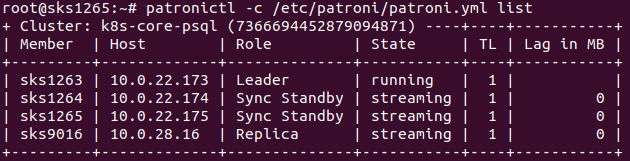
\includegraphics[width=1\linewidth]{source/implementation/construction_implementation/testing/testing_add_pgnode_result}
        \caption{Testing - Patroni Node hinzufügen - add\_pgnode.yml}
        \label{fig:testing_add_pgnode_result}
    \end{figure}
\end{flushleft}